\chapter{State Estimation}
*** Talk about quantifying the performance of the ACS Kalman filter \cite{Sights06}. Discuss training of the covariance matrices. Show the position estimation using the original covariance matrices and the ones found from training. If I get to identifying bias and/or drift in the IMU put that here as well. ***

*** What I really want is plots showing the position estimate using GPS only, KF with learned Q/R but no adapting, KF with no adapting or training, KF with adapting, KF with learned and adaptive, KF with different encoder equations. Would be cool to plot these on an overhead image of the test area. ***

Space and Naval Warfare Systems Center, San Diego (SSC-SD) robotics group has developed the Autonomous Capabilities Suite (ACS) which incorporates many different technologies into a single package that can be run on a wide variety of different robots \cite{Sights06}. One of the ACS libraries is the adaptive extended Kalman filter which is used on the EOD robots for state estimation and is the main method used for answering the question ``Where am I?''. The idea behind the Kalman filter is relatively straightforward. The robot has some basic idea of where it is in the world but there is some uncertainty involved in that estimate due to noise in the sensor measurements and an imperfect model of how the robot moves through the world. Some of the uncertainty of the model can be explained by the fact that not all of the necessary measurements are being carried out and the states can are unobservable. *** Say more here about noise/uncertainty. ***

An example is when the robot is driving in a straight line the left track may be moving on a flat surface while the right track is moving on an uneven surface as in Figure \ref{fig:topography}. The wheel encoders that measure how far each track is moving will report that the right track is traveling a greater distance than the left track which could mean that the robot is turning counter-clockwise or that the robot tracks are moving over different surface types. At the same time the robot will be getting measurements about its heading from both the IMU and GPS sensors that will have some noise as well. In this example both the IMU and GPS sensors would likely say that the robot is traveling in a straight line on average (as long as the controller is performing adequately). The job of the Kalman filter is to determine how much each sensor should be trusted when trying to determine where the robot really is in the world and how fast it is moving. This is accomplished by looking at each of the noise parameters for both the system model and the measurements as being zero mean, white noise, uncorrelated, Gaussian variables ... *** Clean up this language. ***

\begin{figure}[ht!]
	\centering
	
\includegraphics[width=.5\textwidth]{images/topography}
	\caption{Different topographies for the left track and the right track when the ground is smooth on the left side and bumpy on the right side. The top line is for the left track and the bottom line is for the right track.}
	\label{fig:topography}
\end{figure}

\section{The Kalman Filter}
Kalman filters, and even control systems (see Chapter \ref{sec:controls}), use the idea of a state space to encapsulate all of the relevant information that is known about a system such as position, orientation, velocity and acceleration. The standard equations to describe the state space of a system are
\begin{align}
\label{eq:statespace}
\begin{split}
\dot{x} &= f(x,u,t) \\
\dot{y} &= h(x,t)
\end{split}
\end{align}

The ACS Kalman filter is typical of all Kalman filters in that it consists of a prediction update step and a measurement update step where the prediction update is run as fast as possible and the measurement update is run whenever new sensor data becomes available as in Figure \ref{fig:kf}. The prediction update step uses the model of the dynamics of the system and a measurement of elapsed time to determine where the system is in the world. The measurement update step is basically a feedback step to help correct for errors in the system model \cite{Kelly_1994_338}.

\begin{figure}[ht!]
	\centering
	\includegraphics[width=.4\textwidth]{images/kf}
	\caption{The Kalman filter algorithm.}
	\label{fig:kf}
\end{figure}

From \cite{Kelly_1994_338}, \cite{Simon06OptimalEstimation} the prediction update step marches the system dynamics forward in time using the equations
\begin{align}
\label{eq:predictionupdate}
\begin{split}
\hat{x}_{k+1}^- &= \Phi_k\hat{x}_k \\
P_{k+1}^- &= \Phi_kP_k\Phi_k^T + \Gamma_kQ_k\Gamma_k^T
\end{split}
\end{align}
and the measurement update step provides feedback from sensor data using the equations
\begin{align}
\label{eq:measurementupdate}
\begin{split}
K_k &= P_k^-H_k^T\left[H_kP_k^-H_k^T + R_k\right]^{-1} \\
\hat{x}_k &= \hat{x}_k^- + K_k\left[z_k - H_k\hat{x}_k^-\right] \\
P_k &= \left[I - K_kH_k\right]P_k^-
\end{split}
\end{align}

The state space equations for the robot are
\begin{align}
\label{eq:discretess}
\begin{split}
x_{k+1} &= \Phi_kx_k + \Gamma_kw_k \\
z_k &= H_kx_k + v_k
\end{split}
\end{align}

\section{Adaptive Extended Kalman Filter}
*** I really need to clean up the language here. \cite{Busse03adaptiveEKF} looks like a great source. Even the notation as far as \textit{a priori} and \textit{a posteriori} needs fixing. *** Attempting to determine the proper values for the covariance matrices $Q$ in (\ref{eq:predictionupdate}) and $R$ in (\ref{eq:measurementupdate}) can be a laborious process and is often considered more of an art than a science with engineer experience being a critical factor. *** Discuss why $Q$ and $R$ are important and what function they serve in the Kalman filter. *** The ACS Kalman filter has been implemented with an adaptive scheme to update the covariance matrices in real time as the robot moves around and sensor measurements are taken into account \cite{Sights06}, \cite{Mehra72}, \cite{Busse03adaptiveEKF}. $Q$ and $R$ are updated at alternating time steps in the EKF.

The first step is to calculate $Q^\ast$ using
\begin{align}
\label{eq:qstar}
Q^\ast = \left(x-x_{k+1}^-\right)\left(x-x_{k+1}^-\right)^T + P_{k+1}^- - P - Q
\end{align}
Then $Q$ can be updated using
\begin{align}
\label{eq:q}
Q = Q + \frac{1}{L_Q}\left(Q^\ast-Q\right)
\end{align}

Next $R^\ast$ is calculated using
\begin{align}
\label{eq:rstar}
R^\ast = \left(y-Hx\right)\left(y-Hx\right)^T - HP_{k+1}^-H^T
\end{align}
and $R$ can be updated using
\begin{align}
\label{eq:r}
R = R + \frac{1}{L_R}\left(R^\ast-R\right)
\end{align}

*** Discuss the implications of the adaptive EKF. ***

\section{Discriminative Training of Kalman Filter Parameters}
*** Investigate the difference between adaptive filtering and training. It seems like they accomplish the same thing, namely, convergence to some values for the covariance matrices. Do they use the same metrics? Do they converge to the same covariance matrices? Is it just online vs. offline training? *** \cite{Abbeel-RSS-05} describes a method to automatically learn what the covariance matrices should be. When used in conjunction with the adaptive EKF scheme this could allow for faster convergence times when the robots are started and for smaller ranges for the adaptation coefficients $L_Q$ and $L_R$ in (\ref{eq:q}) and (\ref{eq:r}).

\section{Identifty IMU Parameters}